\documentclass{article}

\usepackage{booktabs}
\usepackage{multirow}
\usepackage{amsmath}
\usepackage{hyperref}
\usepackage{overpic}
\usepackage{amssymb}
\usepackage{subcaption}

\usepackage[accepted]{dlai2024}


\begin{document}

\twocolumn[
%%% STUDENTS: FILL IN WITH YOUR OWN INFORMATION
\dlaititle{Per-Sample Amnesiac Unlearning}

\begin{center}\today\end{center}

\begin{dlaiauthorlist}
%%% STUDENTS: FILL IN WITH YOUR OWN INFORMATION
\dlaiauthor{Davide Marincione}{}
\end{dlaiauthorlist}

%%% STUDENTS: FILL IN WITH YOUR OWN INFORMATION
\dlaicorrespondingauthor{Davide Marincione}{marincione.1927757@studenti.uniroma1.it}

\vskip 0.3in
]

\printAffiliationsAndNotice{}

\begin{abstract}
Typical machine unlearning techniques do not scale well with modern deep learning models, as these either require models to abide to strict theoretical guarantees (lowering their effectiveness) or be retrained (unfeasible for big models). In this project we propose a variation of Amnesiac Unlearning, a technique which promises to bring unlearning with little to no compromises to neural networks. Our method lowers the memory requirements of the original technique while maintaining its effectiveness. We test it on MNIST and CIFAR-100, showing that it can make a model forget classes while maintaining its performance on the rest of the dataset.
\end{abstract}
\section{Introduction}
Machine Unlearning is an ever-more important topic in the field of Machine Learning. Not only because privacy concerns regarding deep learning techniques are increasing, but also because regulations such as the EU's GDPR oblige companies to delete user's data at their request. Because of this, research in trying to produce an unlearning procedure that requires the less possible amount of retraining is ongoing.

Our work consists of:
\begin{itemize}
    \item A new unlearning technique with lower memory requirements than the original Amnesiac Unlearning \cite{graves2021amnesiac}.
    \item Tests on MNIST and CIFAR-100 showing that our technique can successfully forget whole classes while maintaining performance on the rest of the dataset.
\end{itemize}
Code can be found at \url{https://github.com/Davide-F5-Marincione/per-sample-amnesiac-unlearning}{https://github.com/Davide-F5-Marincione/per-sample-amnesiac-unlearning}.
\vfill

\section{Related Work}
As far as single-technique driven methods go (combined procedures are often used in practice), the \emph{model shifting} \cite{xu2023survey} family is one of the most promising. These techniques are based on the idea of directly updating a model's parameters to offset the impact of the samples to forget; by finding an update $\delta$ for $w_u=w+\delta$, where $w$ are the parameters of the original model. %The reason for why this solution is so promising is that it does not require a major retraining of the model, which is often infeasible for big models: both in terms of time and computational resources.

One of the most successful \emph{model shifting} techniques is Amnesiac Unlearning \cite{graves2021amnesiac}, which identifies $\delta$ with the updates in which the samples to forget took part. To do so, the parameters' differences are stored on disk, leading to a high memory requirement, as each update is of the same size as the model. %This is a major drawback, as it makes the technique unfeasible for big models.
A recent work \cite{gogineni2024efficient} proposes Layer Unlearning, an approximation which only stores a random subset of the parameters' differences, reducing the memory requirements while decreasing the effectiveness of the technique, and requiring a short retraining phase.

\section{Method}
Our method, similar to \cite{gogineni2024efficient}, consists in storing the gradients for each sample. On the long run, this leads to a lower memory requirement than \cite{graves2021amnesiac}, as it only stores a single subset of parameters for each sample (rather than a new one for each batch). For \cite{graves2021amnesiac}, the space requirements are $O(NM\frac{E}{B})$, whereas for ours it is $O(NMp)$; where $N$ is the number of samples in the dataset, $E$ is the number of epochs, $B$ is the batch size, $M$ is the number of parameters in the model, and $p$ is the percentage of parameters kept in the random subset. Then, if $p<\frac{E}{B}$, our technique requires less memory than the original.

Furthermore, as it only updates with the gradients of the specific samples to forget (rather than the difference imputed by whole batches), our technique has the potential to execute a more 'precise surgery' than both \cite{graves2021amnesiac, gogineni2024efficient}.

\begin{table}
    \centering
    \caption{MNIST with a small CNN, forgetting class $3$. Results are the accuracy of the forgotten class and of the rest of the dataset (in the form 'forgotten/rest').}
    \label{tab:mnist_small_cnn}
    \begin{tabular}{l | c | c c}
        Technique&After train&No retrain&After retrain\\
        \hline
        Original&$0.67$/$0.98$& $0.00$/$0.83$& $0.00$/$0.98$\\
        Layer, $p=.1$&$0.56$/$0.98$& $0.07$/$0.98$& $0.02$/$0.98$\\
        \hline
        Ours, $p=.1$&$0.60$/$0.98$& $0.00$/$0.83$& $0.04$/$0.98$\\
        Ours, $p=.075$&$0.63$/$0.98$&$0.03$/$0.96$& $0.03$/$0.98$\\
        Ours, $p=.05$&$0.60$/$0.98$&$0.06$/$0.96$&$0.04$/$0.98$\\
        Ours, $p=.01$&$0.57$/$0.98$&$0.52$/$0.98$&$0.04$/$0.98$\\
    \end{tabular}
\end{table}

\section{Experiments} We modify the code of \cite{graves2021amnesiac} to test our method, as well as the original \cite{graves2021amnesiac}, and the approximation \cite{gogineni2024efficient} (as they have not published their own code).

Our implementation slightly differs from the original; as in that, the difference between the model before and after the optimization step is used for unlearning, making it invariant to the choice of optimizer. In ours, we directly store the gradients of the model with respect to the loss for each sample; implying that our implementation is not invariant to the choice of optimizer. Still, as in \cite{graves2021amnesiac}, we trained the model with \texttt{Adam} and nonetheless achieved comparable results, therefore we believe this to not be a drawback.

\begin{table}
    \centering
    \caption{CIFAR100 with a small CNN, forgetting class $81$.}
    \label{tab:cifar_small_cnn}
    \begin{tabular}{l | c | c c}
        Technique&After train&No retrain&After retrain\\
        \hline
        Original&$0.17$/$0.33$&$0.00$/$0.04$&$0.00$/$0.35$\\
        Layer, $p=.1$&$0.19$/$0.33$&$0.00$/$0.32$&$0.00$/$0.35$\\
        \hline
        Ours, $p=.1$&$0.24$/$0.33$&$0.00$/$0.14$&$0.00$/$0.36$\\
        Ours, $p=.075$&$0.23$/$0.33$&$0.00$/$0.19$&$0.00$/$0.36$\\
        Ours, $p=.05$&$0.22$/$0.33$&$0.00$/$0.23$&$0.00$/$0.36$\\
        Ours, $p=.01$&$0.24$/$0.33$&$0.04$/$0.32$&$0.00$/$0.36$\\
    \end{tabular}
\end{table}

As a note, we use \texttt{call\_for\_per\_sample\_grads}; which can't work with \texttt{BatchNorm2d}, therefore we modify the standard ResNet-18 implementation by replacing each instance with \texttt{GroupNorm}.

\begin{table}
    \centering
    \caption{MNIST with ResNet-18, forgetting class $3$.}
    \label{tab:mnist_resnet}
    \begin{tabular}{l | c | c c}
        Technique&After train&No retrain&After retrain\\
        \hline
        Original&$0.78$/$0.99$&$0.00$/$0.97$&$0.00$/$0.99$\\
        Layer, $p=.1$&$0.83$/$0.99$&$0.69$/$0.99$&$0.00$/$0.99$\\
        \hline
        Ours, $p=.2$&$0.81$/$0.99$&$0.24$/$0.97$&$0.00$/$0.99$\\
        Ours, $p=.1$&$0.85$/$0.98$&$0.73$/$0.97$&$0.00$/$0.99$\\
        Ours, $p=.075$&$0.83$/$0.98$&$0.77$/$0.98$&$0.02$/$0.99$\\
    \end{tabular}
\end{table}

We test our method on MNIST and CIFAR-100, with a small CNN and a ResNet-18. During all tests, we run the training for $4$ epochs (the maximum epochs that the original technique can run without going OOM on a Kaggle Notebook) and the retraining (without the forgotten data) for $4$ epochs too.
From these, we see that our technique can roughly achieve the same results of \cite{gogineni2024efficient} with a lower $p$, and that, despite being the more complex dataset, CIFAR-100 is the one where our technique can get more efficient (reaching a lower $p$ while keeping the performance on the forget class low).

\begin{table}
    \centering
    \caption{CIFAR100 with ResNet-18, forgetting class $81$. ($^\dagger$) Had to sum differences into single dictionary, otherwise going OOM.}
    \label{tab:cifar_resnet}
    \begin{tabular}{l | c | c c}
        Technique&After train&No retrain&After retrain\\
        \hline
        Original$^\dagger$&$0.18$/$0.33$&$0.00$/$0.02$&$0.00$/$0.41$\\
        Layer$^\dagger$, $p=.1$&$0.12$/$0.32$&$0.00$/$0.30$&$0.00$/$0.39$\\
        \hline
        Ours, $p=.1$&$0.21$/$0.33$&$0.00$/$0.17$&$0.00$/$0.41$\\
        Ours, $p=.075$&$0.16$/$0.34$&$0.00$/$0.23$&$0.00$/$0.40$\\
        Ours, $p=.05$&$0.15$/$0.33$&$0.00$/$0.30$&$0.00$/$0.40$\\
        Ours, $p=.025$&$0.22$/$0.33$&$0.01$/$0.31$&$0.00$/$0.40$\\
        Ours, $p=.01$&$0.18$/$0.33$&$0.11$/$0.33$&$0.00$/$0.40$\\
    \end{tabular}
\end{table}

In \cite{graves2021amnesiac} a Model Inversion Attack \cite{fredrikson2015inversion} is tried on their technique; they find it to be working. We try it too, and likewise find our technique to be lacking, probably even more as we change just part of the parameters.

\begin{figure}
    \centering
    \begin{subfigure}[b]{0.23\textwidth}
        \centering
        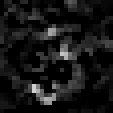
\includegraphics[width=.48\textwidth]{trained_single.png}
        \caption{After training.}
    \end{subfigure}%
    \begin{subfigure}[b]{0.23\textwidth}
        \centering
        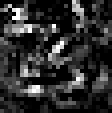
\includegraphics[width=.48\textwidth]{retrained_single.png}
        \caption{After retraining.}
    \end{subfigure}
    \caption{Inversion Attack on ResNet-18 for class $3$ of MNIST and $p=.25$. Even with such a high $p$ and retraining, the inversion attack is successful.}
    \label{fig:inversion}
\end{figure}

\section{Conclusion}
We've empirically shown that amnesiac unlearning can be even more powerful if done per-sample rather than per-batch. Furthermore, we can effectively unlearn training samples by modifying just a fraction of the model's parameters. Thanks to these two properties, our technique has the potential to be more effective than the approximation proposed in \cite{gogineni2024efficient}. Further work could be done to find the optimal subset of parameters to keep, rather than using a random subset. One could make it more efficient by compressing the representation of the gradients themselves using lower bit precision and other techniques.

\bibliography{references.bib}
\bibliographystyle{dlai2024}

\end{document}